\section{为什么选择 \ttfamily{Kotlin}}%
\begin{frame}[fragile]
    \frametitle{历史}
    \begin{columns}
        \begin{column}{0.5\textwidth}
            \begin{itemize}
                \item \textbf{2011} |JetBrains| 发布,面向 JVM
                \item \textbf{2016} |v1.0| 发布
                \item \textbf{2017} \google{} 宣布在{\color{android}\faAndroid}Android 提供 Kotlin 的最佳支持
                \item \textbf{2019} 已作为{\color{android}\faAndroid}Android 开发的推荐语言
            \end{itemize}
        \end{column}
        \begin{column}{0.5\textwidth}
            \begin{figure}
            \begin{center}
                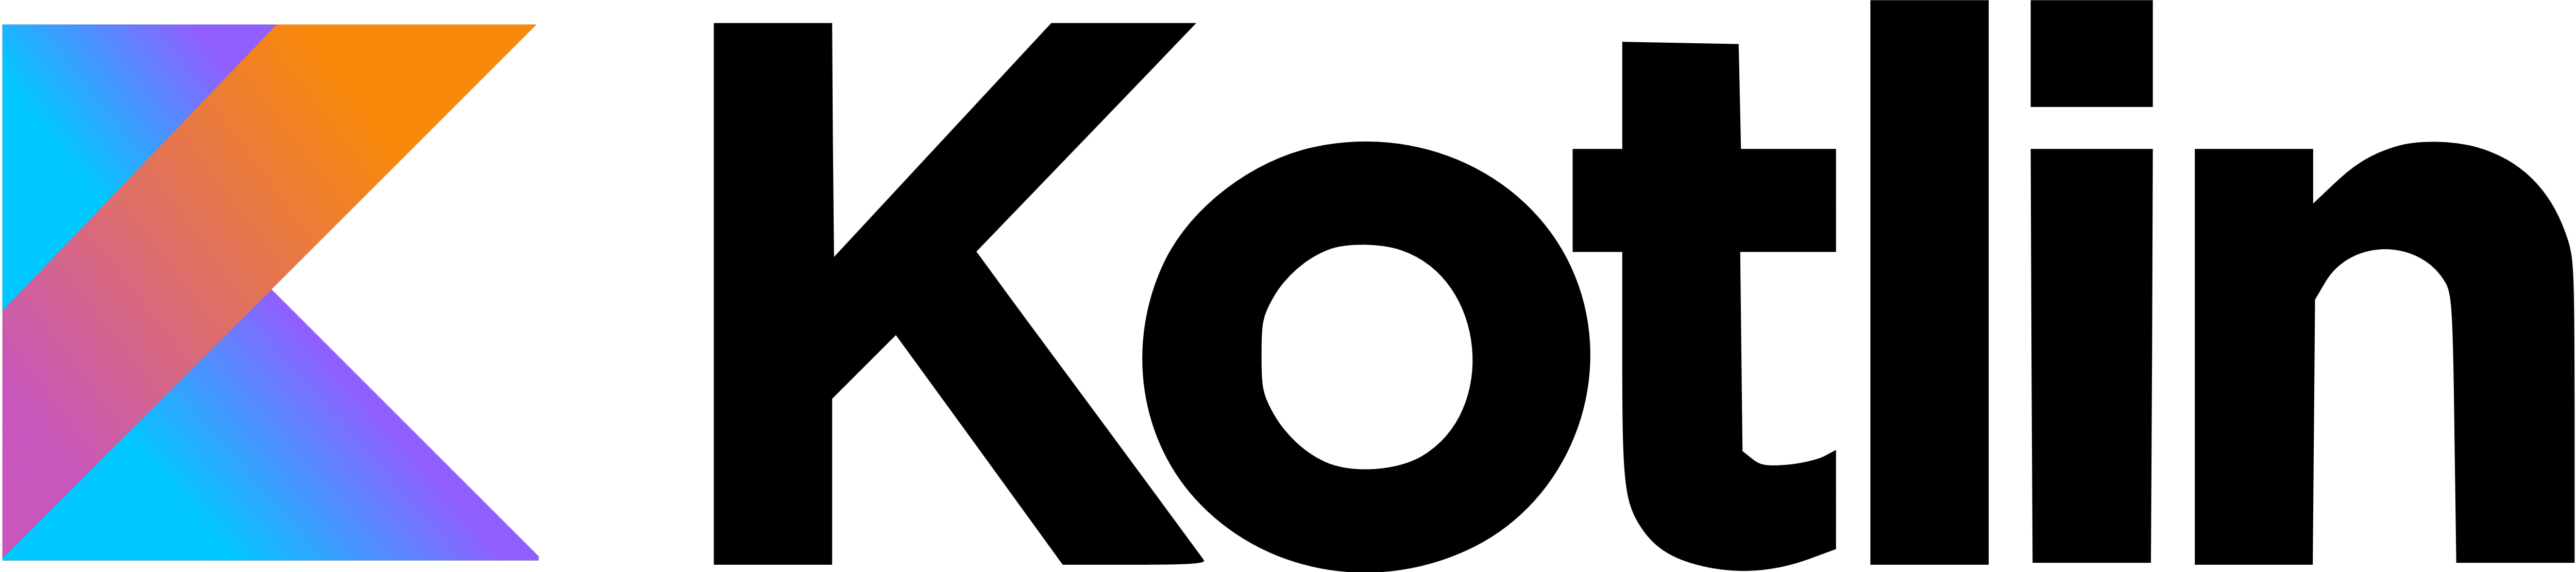
\includegraphics[height=1cm]{fig/Kotlin}\\
                \vspace{12pt}
                
\includegraphics[height=2cm]{fig/android}
            \end{center}
            \end{figure}
        \end{column}
    \end{columns}
\end{frame}

\begin{frame}[t,fragile]
    \frametitle{特性}
    \begin{quotebox}
        让开发人员更快乐的一门现代编程语言$^1$。
    \end{quotebox}
    \nonumberfootnote{$^1$出自 Kotlin 语言中文站\link{https://www.kotlincn.net/}}
    \vspace{12pt}
    \begin{columns}[t]
        \begin{column}{0.4\textwidth}
            \begin{block}{\faCut{} 简洁}
                数据类\\
                函数式编程\\
                单例
            \end{block}
        \end{column}
        \begin{column}{0.4\textwidth}
            \begin{block}{\faHardHat{} 安全}
                空安全\\
                自动类型转换
            \end{block}
        \end{column}
    \end{columns}
    \begin{columns}[t]
        \begin{column}{0.4\textwidth}
            \begin{block}{\faPuzzlePiece{} 互操作性}
                Java\\
                Android
            \end{block}
        \end{column}
        \begin{column}{0.4\textwidth}
            \begin{block}{\faWrench{} 工具友好}
                Java IDE\\
                命令行\\
                Jupyter
            \end{block}
        \end{column}
    \end{columns}
\end{frame}

\begin{frame}[fragile]
    \frametitle{\texttt{Why Kotlin?}}
    \begin{columns}
        \begin{column}{0.5\textwidth}
            \begin{itemize}
                \item 越来越多应用通过 |Kotlin| 开发
                \item 用更\textcolor{penroseblue}{短}的代码写出更\textcolor{penroseblue}{安全}的应用
                \item 学习现代编程语言的新特性\\类型推断、函数式编程、协程……
            \end{itemize}
        \end{column}
        \begin{column}{0.5\textwidth}
            \begin{figure}
            \begin{center}
                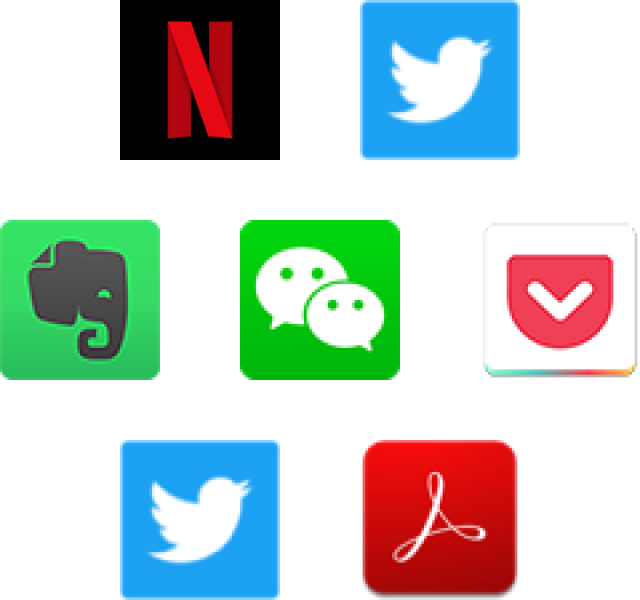
\includegraphics[height=3cm]{fig/apps.png}
            \end{center}
            \end{figure}
        \end{column}
    \end{columns}
\end{frame}
